% !TEX program = pdflatex
\documentclass[aspectratio=169]{beamer}

% ======================
% THEME & LANG
% ======================
\usetheme{Madrid}
\usecolortheme{default}
\useinnertheme{rounded}
\usefonttheme{professionalfonts}

\usepackage[english]{babel}
\usepackage[utf8]{inputenc}
\usepackage[T1]{fontenc}
\usepackage{lmodern}

% ======================
% PACKAGES
% ======================
\usepackage{graphicx}
\usepackage{booktabs}
\usepackage{tabularx}
\usepackage{array}
\usepackage{multicol}
\usepackage{pgfplots}
\pgfplotsset{compat=1.18}
\usepackage{pgf-pie}
\usepackage{tikz}
\usetikzlibrary{arrows.meta,positioning,shapes.geometric,fit,calc}

% ======================
% META
% ======================
\title[CA + GA for Urban Growth]{Evolutionary Model of Urban Growth with Cellular Automata + Genetic Algorithms}
\subtitle{Thesis progress and literature review synthesis}
\author{Rodrigo Moreno López}
\institute{IIMAS--UNAM}
\date{September 5, 2025}

% ======================
% MACROS (adjust here the counts of the bibliography)
% ======================
\newcommand{\TotalRefs}{31}
\newcommand{\RefsCA}{10}
\newcommand{\RefsCalib}{6}
\newcommand{\RefsRS}{8}
\newcommand{\RefsImpacto}{4}
\newcommand{\RefsTools}{3}
% Safe derived values for PGFPlots (avoid arithmetic in restricted mode)
\pgfmathtruncatemacro{\RefsOthers}{\TotalRefs-\RefsCalib}
\pgfmathtruncatemacro{\YMax}{\TotalRefs+2} 


% ======================
% DOCUMENTO
% ======================
\begin{document}

% TÍTULO
\begin{frame}
  \titlepage
\end{frame}

% AGENDA
\begin{frame}{Agenda}
  \tableofcontents
\end{frame}

\section{Contexto}
\begin{frame}{Contexto y Problema}
  \begin{itemize}
    \item El crecimiento urbano en México y en el mundo ejerce presión sobre ecosistemas, infraestructura y calidad de vida.
    \item Los \textbf{Autómatas Celulares (AC)} son efectivos para capturar dinámicas espaciales a partir de reglas locales.
    \item Reto: \textbf{calibración} de parámetros (pesos de influencia, umbrales, factores espaciales) de forma reproducible y no sesgada.
    \item Propuesta: \textbf{AC + Algoritmo Genético (AG)} con inicialización guiada por \emph{Weight of Evidence (WoE)} y validación con métricas espaciales.
  \end{itemize}
\end{frame}

\section{Objetivos}
\begin{frame}{Objetivo General}
  \large
  Desarrollar un \textbf{modelo evolutivo AC+AG} para simular y \textbf{predecir} el crecimiento urbano de una región específica, optimizando parámetros con datos satelitales históricos.
\end{frame}

\begin{frame}{Objetivos Específicos}
  \begin{enumerate}
    \item Implementar un AC binario/multinivel para cambio de uso de suelo.
    \item Integrar un AG para la calibración automática de \emph{pesos}, \emph{umbrales} y \emph{factores espaciales}.
    \item Procesar y clasificar series temporales satelitales; calcular \textbf{WoE} para extracción de conocimiento espacial.
    \item Validar con métricas (IoU, FOM, Kappa) y análisis temporal/espacial.
    \item Explorar escenarios de crecimiento (políticas, restricciones, transporte).
  \end{enumerate}
\end{frame}

\section{Estado del Arte}
\begin{frame}{Estado del Arte: Síntesis}
  \begin{itemize}
    \item \textbf{AC y SLEUTH}: robustos pero requieren calibración manual intensiva.
    \item \textbf{Optimización evolutiva}: AG/PSO/MOO para calibración de AC mejoran la concordancia con datos reales.
    \item \textbf{Sensado remoto}: Landsat/Sentinel y DL permiten insumos multitemporales de alta calidad.
    \item \textbf{Tendencia tecnológica}: ecosistema de código abierto (DEAP, Repast, UrbanSim, PyLUSAT) que habilita reproducibilidad.
  \end{itemize}
\end{frame}

\begin{frame}{Comparación de Enfoques}
  \scriptsize
  \begin{tabularx}{\textwidth}{>{\bfseries}l X X >{\raggedright\arraybackslash}p{1.9cm}}
    \toprule
    Enfoque & Fortalezas & Debilidades & Métricas \\
    \midrule
    SLEUTH & Robusto, probado en múltiples regiones & Calibración manual intensiva; dependiente del modelador & Kappa, FOM \\
    AC + AG + SLEUTH & Calibración automática; ablations; reproducible & Costo computacional; ajuste de hiperparámetros & IoU, FOM \\
    AC + DL & Aprende reglas complejas a partir de datos & Requiere gran cantidad de etiquetas y cómputo & IoU, AUC \\
    \bottomrule
  \end{tabularx}
\end{frame}

\section{Bibliografía Revisada}
\begin{frame}{Cobertura Bibliográfica (\TotalRefs~fuentes)}
  \vspace{-0.6em}
      \textbf{Distribución temática}
      \vspace{0.3em}
      \begin{center}
        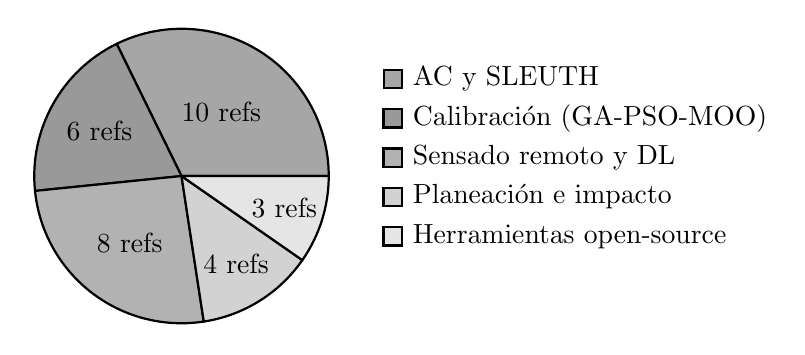
\begin{tikzpicture}[scale=0.85]
          \pie[
            sum=auto,
            after number=~refs,
            radius=2.2,
            text=legend,
            color={gray!70,gray!80,gray!60,gray!35,gray!20},
            /tikz/every text node part/.style={align=left}
          ]{
            \RefsCA/AC y SLEUTH,
            \RefsCalib/Calibración (GA-PSO-MOO),
            \RefsRS/Sensado remoto y DL,
            \RefsImpacto/Planeación e impacto,
            \RefsTools/Herramientas open-source
          }
        \end{tikzpicture}
      \end{center}
\end{frame}

\begin{frame}{Algunos Hallazgos}
      \textbf{Hallazgos}
      \vspace{0.3em}
      {\small
      \begin{itemize}
        \item La literatura está dominada por \textbf{AC/SLEUTH} y \textbf{sensado remoto}.
        \item La \textbf{calibración automática} con AG/MOO es una línea en crecimiento.
        \item El ecosistema \textbf{open-source} habilita replicabilidad y transferencia tecnológica.
      \end{itemize}}
\end{frame}

\begin{frame}{¿Cuántos artículos tratan directamente con AC+AG?}
  \begin{center}
    \begin{tikzpicture}
      \begin{axis}[
        ybar,
        bar width=28pt,
        ymin=0,
        ymax=\YMax,
        width=0.8\textwidth,
        height=0.5\textheight,
        symbolic x coords={AC+AG,Otros temas},
        xtick=data,
        nodes near coords,
        nodes near coords align={vertical},
        ylabel={Número de referencias},
        ymajorgrids=true,
        grid style=dashed
      ]
        \addplot coordinates {(AC+AG,\RefsCalib) (Otros temas,\RefsOthers)};
      \end{axis}
    \end{tikzpicture}
  \end{center}
  \vspace{-0.6em}
  \centering
  \footnotesize Ejemplos: Almeida (2003), Li \& Dang (2013), Huang (2019), Wang (2021), Tang (2024).
\end{frame}

\section{Metodología Propuesta}
\begin{frame}{Pipeline Metodológico (propuesto)}
  \begin{center}
  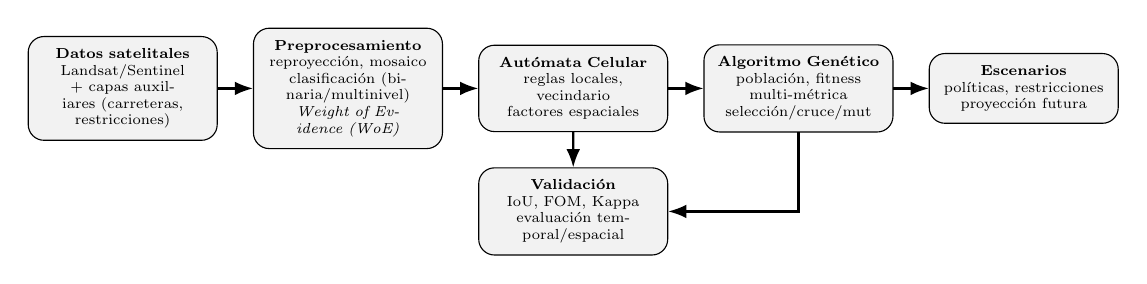
\begin{tikzpicture}[
      node distance=6mm and 6mm,
      every node/.style={font=\scriptsize},
      box/.style={
        draw, rounded corners=2mm, align=center, inner sep=2mm, fill=gray!10,
        text width=2.8cm, minimum height=1cm
      },
      >={Latex},
      scale=0.75, transform shape
    ]
    % NODOS
    \node[box] (datos) {\textbf{Datos satelitales}\\Landsat/Sentinel\\+ capas auxiliares (carreteras, restricciones)};
    \node[box, right=of datos] (prep) {\textbf{Preprocesamiento}\\reproyección, mosaico\\clasificación (binaria/multinivel)\\\emph{Weight of Evidence (WoE)}};
    \node[box, right=of prep] (ca) {\textbf{Autómata Celular}\\reglas locales, vecindario\\factores espaciales};
    \node[box, right=of ca] (ga) {\textbf{Algoritmo Genético}\\población, fitness multi-métrica\\selección/cruce/mut};

    \node[box, below=of ca] (val) {\textbf{Validación}\\IoU, FOM, Kappa\\evaluación temporal/espacial};
    \node[box, right=of ga] (esc) {\textbf{Escenarios}\\políticas, restricciones\\proyección futura};

    % FLECHAS
    \draw[->, thick] (datos) -- (prep);
    \draw[->, thick] (prep) -- (ca);
    \draw[->, thick] (ca) -- (ga);
    \draw[->, thick] (ga) -- (esc);
    \draw[->, thick] (ca) -- (val);
    \draw[->, thick] (ga) |- (val);
  \end{tikzpicture}
  \end{center}
\end{frame}


\section{Impacto}
\begin{frame}{Impacto Esperado}
  \begin{columns}[T]
    \begin{column}{0.33\textwidth}
      \textbf{Científico}
      \begin{itemize}
        \item Cierra la brecha en \emph{calibración reproducible} de AC.
        \item Integra WoE + AG + métricas espaciales.
        \item Código abierto y pipelines modulares.
      \end{itemize}
    \end{column}
    \begin{column}{0.33\textwidth}
      \textbf{Social}
      \begin{itemize}
        \item Apoya la planeación urbana y conservación.
        \item Sensibilidad a escenarios y restricciones.
        \item Transparencia para tomadores de decisiones.
      \end{itemize}
    \end{column}
    \begin{column}{0.33\textwidth}
      \textbf{Tecnológico}
      \begin{itemize}
        \item Uso de \textbf{open-source}: DEAP, Repast, UrbanSim, PyLUSAT.
        \item Escalable en GPU/cluster.
        \item Integrable con SIG modernos.
      \end{itemize}
    \end{column}
  \end{columns}
\end{frame}

\section{Diferenciadores}
\begin{frame}{¿Qué aporta esta tesis? (\emph{Diferenciadores})}
  \begin{itemize}
    \item \textbf{Extracción de conocimiento} (WoE) para guiar la búsqueda evolutiva.
    \item \textbf{Calibración multi-métrica} (IoU/FOM/Kappa) y ablations por factores.
    \item \textbf{Reproducibilidad de extremo a extremo} (datos \textrightarrow{} código \textrightarrow{} resultados).
    \item \textbf{Escenarios de política pública} y evaluación de trade-offs espaciales.
  \end{itemize}
\end{frame}

\section{Próximos Pasos}
\begin{frame}{Plan para el Próximo Trimestre}
  \begin{enumerate}
    \item Consolidar conjunto de entrenamiento/validación con series temporales (limpieza y QA).
    \item Implementar módulo base AC + WoE y definir cromosoma del AG.
    \item Definir fitness multi-objetivo y criterios de parada.
    \item Experimentos de ablation (vecindario, pesos, restricciones).
    \item Redactar resultados y discusión; liberar repositorio \texttt{open-source}.
  \end{enumerate}
\end{frame}

\section{Conclusión}
\begin{frame}{Conclusión}
  \begin{itemize}
    \item La literatura respalda el \textbf{potencial} de AC + optimización evolutiva para crecimiento urbano.
    \item Esta propuesta enfatiza \textbf{automatización}, \textbf{reproducibilidad} y \textbf{aplicabilidad} a contextos reales en México.
    \item Es un \textbf{tema sólido de tesis de maestría} con impacto científico, social y tecnológico.
  \end{itemize}
\end{frame}

% REFERENCIAS
\appendix
\begin{frame}{Referencias Clave (selección breve)}
  \footnotesize
  \begin{itemize}
    \item Clarke \& Gaydos (1997); Clarke (2007); White \& Engelen (1997); Wolfram (1984).
    \item Almeida et al. (2003); Li \& Dang (2013); Huang et al. (2019); Wang et al. (2021); Tang et al. (2024).
    \item Herold et al. (2003); Gong et al. (2013); Ma et al. (2019); Kadhim et al. (2018).
    \item DEAP (Fortin et al., 2024); Repast (North et al., 2023); UrbanSim (Waddell \& Foti, 2020); PyLUSAT (Miller \& Li, 2022).
    \item Angel (2016); Seto et al. (2011, 2012); ONU-Habitat (2020).
  \end{itemize}
\end{frame}

\end{document}
